\chapter{Syklittömät verkot}

\section{Topologinen järjestys}

Suunnatun verkon \emph{topologinen järjestys} on solmujen järjestys,
jossa pätee, että jos solmusta $a$ on kaari solmuun $b$,
niin solmu $a$ on ennen solmua $b$ järjestyksessä.
Topologinen järjestys voidaan antaa listana,
joka sisältää kaikki verkon solmut sopivassa järjestyksessä.

\begin{figure}
\center
\begin{center}
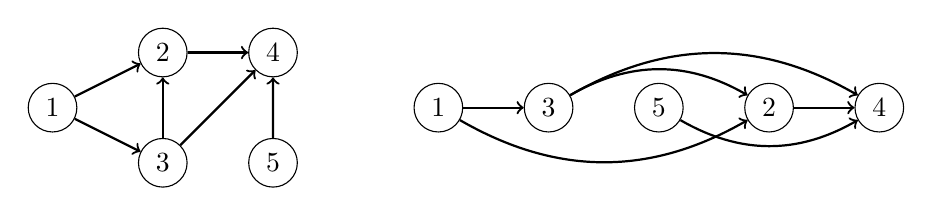
\begin{tikzpicture}[scale=0.7]
\begin{scope}
\node[draw, circle] (1) at (0,-1) {$1$};
\node[draw, circle] (2) at (2,0) {$2$};
\node[draw, circle] (3) at (2,-2) {$3$};
\node[draw, circle] (4) at (4,0) {$4$};
\node[draw, circle] (5) at (4,-2) {$5$};
\path[draw,thick,->] (1) -- (2);
\path[draw,thick,->] (1) -- (3);
\path[draw,thick,->] (3) -- (2);
\path[draw,thick,->] (2) -- (4);
\path[draw,thick,->] (3) -- (4);
\path[draw,thick,->] (5) -- (4);
\end{scope}
\begin{scope}[xshift=7cm]
\node[draw, circle] (1) at (0,-1) {$1$};
\node[draw, circle] (3) at (2,-1) {$3$};
\node[draw, circle] (5) at (4,-1) {$5$};
\node[draw, circle] (2) at (6,-1) {$2$};
\node[draw, circle] (4) at (8,-1) {$4$};
\path[draw,thick,->] (1) edge [bend right] (2);
\path[draw,thick,->] (1) -- (3);
\path[draw,thick,->] (3) edge [bend left] (2);
\path[draw,thick,->] (2) -- (4);
\path[draw,thick,->] (3) edge [bend left] (4);
\path[draw,thick,->] (5) edge [bend right] (4);
\end{scope}
\end{tikzpicture}
\end{center}
\caption{Verkko ja yksi sen topologinen järjestys $[1,3,5,2,4]$.}
\label{fig:topjar}
\end{figure}

Kuvassa \ref{fig:topjar} on esimerkkinä verkko ja sitä vastaava topologinen
järjestys $[1,3,5,2,4]$.
Huomaa, että verkolla on usein monta mahdollista
topologista järjestystä.
Esimerkiksi tässä verkossa myös $[5,1,3,2,4]$,
$[1,5,3,2,4]$ ja $[1,3,2,5,4]$
ovat topologisia järjestyksiä, koska voimme valita monella tavalla,
missä vaiheessa solmu $5$ on järjestyksessä.

Jos suunnattu verkko on syklitön, voimme muodostaa sille
aina topologisen järjestyksen.
Toisaalta jos verkossa on sykli,
topologista järjestystä ei voi olla olemassa,
koska emme voi valita mitään syklissä olevaa solmua
järjestykseen ennen toista.
Seuraavaksi tutustumme algoritmiin,
jonka avulla voimme muodostaa topologisen järjestyksen
tai todeta, että verkossa on sykli eikä järjestys ole mahdollinen.

\subsection{Järjestyksen muodostaminen}

Voimme muodostaa topologisen järjestyksen käyttämällä
muunnettua syvyyshakua, jossa jokaisella solmulla on kolme tilaa:

\begin{itemize}
\item tila 0 (valkoinen): solmussa ei ole käyty
\item tila 1 (harmaa): solmun käsittely on kesken
\item tila 2 (musta): solmun käsittely on valmis
\end{itemize}

Algoritmin alussa jokainen solmu on valkoinen.
Käymme läpi kaikki verkon solmut ja aloitamme aina syvyyshaun
solmusta, jos se on valkoinen.
Aina kun saavumme uuteen solmuun, sen väri muuttuu
valkoisesta harmaaksi.
Sitten kun olemme käsitelleet kaikki solmusta lähtevät
kaaret, sen väri muuttuu harmaasta mustaksi.

Algoritmin aikana luomme listan, johon lisäämme solmun
aina silloin, kun sen väri muuttuu mustaksi.
Tämä lista käänteisessä järjestyksessä on verkon
topologinen järjestys.
Kuitenkin jos saavumme jossain vaiheessa uudestaan harmaaseen solmuun,
verkossa on sykli eikä topologista järjestystä voi muodostaa.

Kuva X näyttää, kuinka algoritmi muodostaa topologisen
järjestyksen esimerkkiverkossamme.
Tässä tapauksessa syvyyshakuja on kaksi,
joista ensimmäinen alkaa solmusta 1 ja toinen alkaa solmusta 5.
Algoritmin tuloksena on lista $[4,2,3,1,5]$,
joten käänteinen lista $[5,1,3,2,4]$ on verkon topologinen järjestys.

\section{Dynaaminen ohjelmointi}

\section{Vahvasti yhtenäisyys}

